\documentclass[12pt]{article}

\usepackage{graphicx}
\usepackage{paralist}
\usepackage{amsfonts}
\usepackage{listings}
\usepackage{hyperref}
\usepackage{tabto}
\usepackage[table]{xcolor}
\usepackage{float}
\usepackage[normalem]{ulem}

\hypersetup{colorlinks=true,
    linkcolor=blue,
    citecolor=blue,
    filecolor=blue,
    urlcolor=blue,
    unicode=false}

\oddsidemargin 0mm
\evensidemargin 0mm
\textwidth 160mm
\textheight 200mm

\pagestyle {plain}
\pagenumbering{arabic}

\newcounter{stepnum}

\usepackage{fancyhdr}
\usepackage{fancyhdr}
\fancyhead[L]{\today\ }
\fancyhead[C]{D2}
\fancyhead[R]{Group 5}
\pagestyle{fancy}

\title{Deliverable 2: Revision 0}
\author{Group 5 \\
		\\ Lu, Daniel - lud1  - 400015933
		\\ Abujarad, Razan - abujarar  - 400038238
		\\ Panunto, Michael - panuntom - 400022970
		\\ Samarasinghe, Sachin - samarya - 001430998
		\\ Bengezi, Mohamed - bengezim - 400021279 \\
		\\ Professor: Dr. Kehdri
		\\ Tutorial: T02}

\begin {document}


% Options to be used by the tables
\setlength{\arrayrulewidth}{1.5pt}
\definecolor{light-gray}{gray}{0.93}

\maketitle

\newpage

{\centering
  \tableofcontents\par
}
\addtocontents{toc}{\protect\vspace{2.5em}}
\newpage

\section{Introduction}
\label{sec:introduction}
% Begin Section

An introduction to the document.

\subsection{Purpose}
This document provides a high level overview of the software architecture of Bookzilla. It describes how Bookzilla's software architecture is chosen to match the problem it solves. It describes how the program is divided into sub-systems and modules based on the components of the software architecture. This document is geared toward any individuals/organizations that has a stake in the implementation and maintenance of Bookzilla (i.e: software engineers, software developers, etc..).
% End SubSection

\subsection{System Description}
Bookzilla is an Android app that searches for books based on the user's description of a book. Search results provided by Bookzilla is an approximation based on the user's description. This is because the description could be too vague or it is inaccurate. Therefore, the software architecture that is used to implement Bookzilla must suit well for approximating solutions.\\

\noindent Blackboard architecture is well-suited for approximating solutions and it is used for implementing Bookzilla. The provided description of the book is provided to different software modules called ``experts``. Each expert specializes in a specific search criteria (i.e: search by author) and provides search results based on that specific criteria. Final result is chosen from the results from the experts by using a selection algorithm.
% End SubSection

\subsection{Overview}
In-addition to the introduction, this document contains a use case diagram with descriptions of use cases, an analysis class diagram, an explanation of the system architecture and class responsibility collaboration (CRC) cards.\\

\noindent Sections of this document follow a logical flow of content that build upon the previous sections. As the document progresses, its content become more implementation oriented.
% End Section

\newpage
\section{Use Case Diagram}
\label{sec:use_case_diagram}
% Begin Section
\begin{figure}[h]
\centering
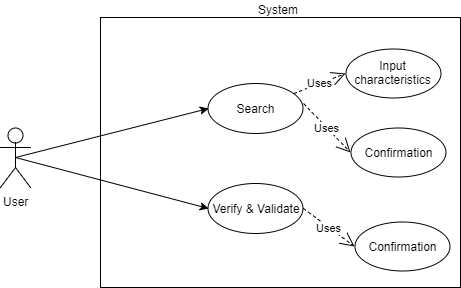
\includegraphics[height=75mm]{UseCase.png}
\caption{Use Case Diagram}
\label{fig:use_case}
\end{figure}
\begin{itemize}
    \item \textbf{Search: } This is where the user initiates the search, inputs the attributes of the book, and confirms \& launches the search
    \begin{itemize}
        \item Input attributes: The method of input allowing the user to define attributes of the book
        \item Confirmation: Finalizing and Launching the search
    \end{itemize}
    \item \textbf{Verify \& Validate: } This is where the user confirms the output given to them by the system.
        \begin{itemize}
        \item Confirmation: Reviewing the list of books outputted by the system using the information given on each book
    \end{itemize}
\end{itemize}
\newpage
% End Section

\section{Analysis Class Diagram}
\label{sec:analysis_class_diagram}
% Begin Section
\begin{figure}[h]
\centering
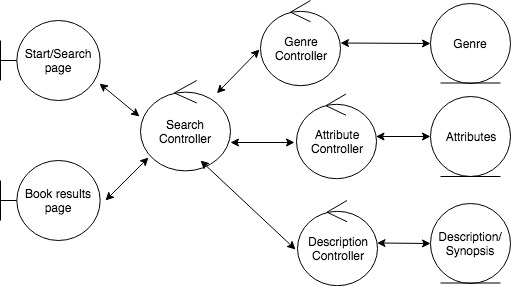
\includegraphics[scale=0.7]{AnalysisClassDiagram.jpeg}
\caption{Analysis Class Diagram}
\label{fig: analysis class diagram}
\end{figure}
% End Section


\section{Architectural Design}
\label{sec:architectural_design}
% Begin Section


\subsection{System Architecture}
\label{sub:system_architecture}
% Begin SubSection
BookZilla implements a blackboard architecture. A user input triggers the search controller; this search controller parses and modifies the user input and passes the information to the expert controller. Upon receiving the parsed information, the expert controller separates the data according to category and sends it to their respective expert. Each expert is able to consult the Google Books API to retrieve a unique list of books based on their expertise. The lists returned from the experts are then sent back to the expert controller which in turn passes the collection of book lists to the results modifier. The results modifier uses this collection to produce a single list containing the subset of common books relating to the user's criteria. This single list is passed to the results page where books are displayed to the user in order of relevance to their query.\\

The purpose of BookZilla is to identify books based on varying forms of search criteria. Through the use of multiple experts, the application is able to find books best suited for the user. A blackboard architecture is an ideal fit for knowledge based systems such as this since they are based on the practice of compiling the partial views provided by knowledgeable experts through the user of a controller to achieve a final, complete solution.

\begin{figure}[h]
\centering
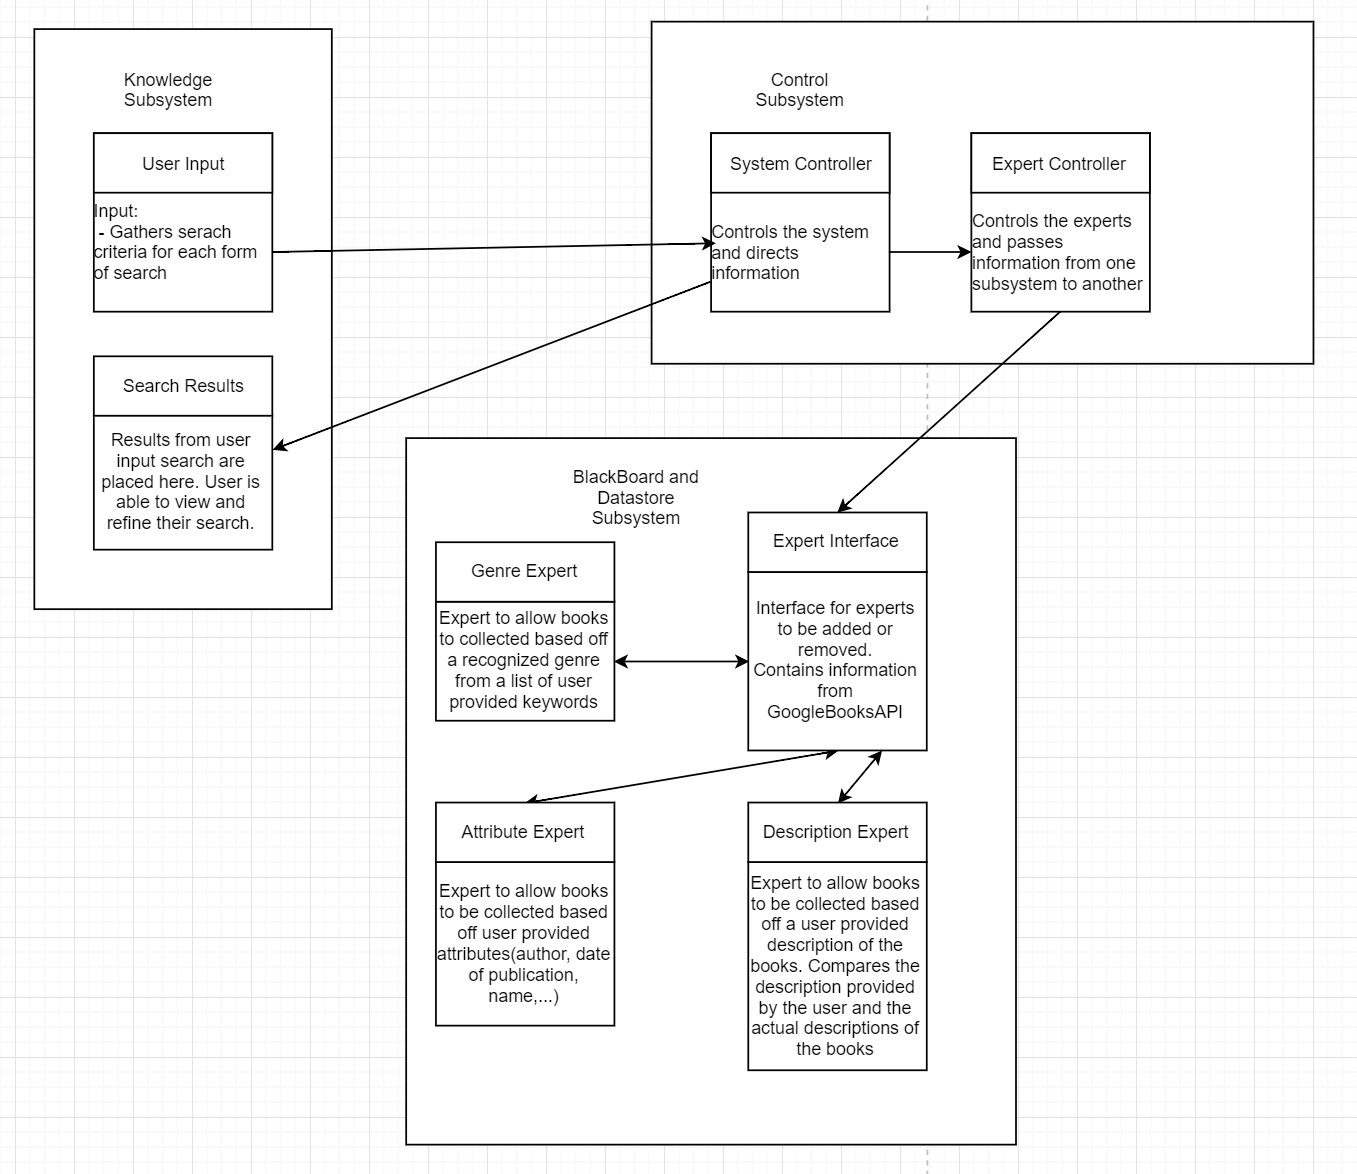
\includegraphics[height=120mm]{SubsystemDiagram.png}
\caption{SubsystemDiagram}
\label{fig:SubsystemDiagram}
\end{figure}

% End SubSection

\subsection{Subsystems}
\label{sub:subsystems}
% Begin SubSection
\subsubsection{Knowledge Subsystem}

The knowledge subsystem consists of the User Input and Search Result pages. It is responsible for guiding users and gathering the user inputted data to be used by the control subsystem. Additionally, the knowledge subsystem retrieves final results from the control subsystem which it then displays for the user on the Search Result page. This subsystem directly interacts with only the control subsystem by passing and retrieving data.

\subsubsection{Control Subsystem}

The control subsystem consists of the Search Controller and the Expert Controller. The Search Controller is responsible for parsing the data received from the knowledge subsystem so that it can be read by the correct expert. The new data is passed along through the Expert controller to the blackboard and data store subsystem. Additionally, the expert controller receives the results returned from the blackboard and data store subsystem, and creates a finalized collection from each of the experts' returned lists which is then sent back through the Search Controller to the knowledge subsystem. The control subsystem interacts with both the knowledge subsystem and the blackboard and data store subsystem, it acts a central system essentially allowing indirect communication between the user and experts.

\subsubsection{Blackboard and Data Store Subsystem}

The blackboard and data store subsystem is the largest subsystem within Bookzilla, it consists of the genre expert, attribute expert, description expert and expert interface. The genre expert determines the genre of the desired book from a user input and returns books that are a possible match. The attribute expert uses data involving the attributes of the book such as approximate page length, author, publication date and so on; books containing all of the attributes are returned from this expert. The description expert takes a user inputted description and returns books with matching keywords. The expert interface is an interface designed for the addition and removal of experts. It also contains information taken from the Google Books API. The blackboard and data store subsystem is used to retrieve and analyze data, before interacting with the control subsystem to return a solution to the user's query.

% End SubSection

% End Section
	
\section{Class Responsibility Collaboration (CRC) Cards}
\label{sec:class_responsibility_collaboration_crc_cards}
% Begin Section
	\begin{table}[H]
		\centering
		\begin{tabular}{|p{5cm}|p{5cm}|}
		\hline 
		 \multicolumn{2}{|l|}{\textbf{MainActivity}} \\
		\hline
		\textbf{Responsibility:} & \textbf{Collaborators:} \\
		\hline
		 Display welcome message and application information & \\
		\hline
		Display a button to initiate search & \\
		\hline
		Transfer user to to search page & SearchActivity \\
		\hline
		\end{tabular}
	\end{table}
	

	\begin{table}[H]
		\centering
		\begin{tabular}{|p{5cm}|p{5cm}|}
		\hline 
		 \multicolumn{2}{|l|}{\textbf{Class Name:SearchActivity}} \\
		\hline
		\textbf{Responsibility:} & \textbf{Collaborators:} \\
		\hline
		Display required expert sections titles & \\
		\hline
		Display input box for Genre & \\
		\hline
		Display input box for Description & \\
		\hline
		Display input boxes for book attributes & \\
		\hline
		%modified controllers 
		Send received inputs to the Search controller & Genre Controller, Attribute Controller and Description Controller \\
		\hline
		\end{tabular}
	\end{table}
	
	\begin{table}[H]
		\centering
		\begin{tabular}{|p{5cm}|p{5cm}|}
		\hline 
		 \multicolumn{2}{|l|}{\textbf{Class Name: GenreExpert}} \\
		\hline
		\textbf{Responsibility:} & \textbf{Collaborators:} \\
		\hline
		 Receive information from Genre Controller & Genre Controller \\
		\hline
		 Use input Genre to search for books & GoogleAPI \\
		 \hline
		 Compile a list of viable books & \\
		 \hline
		 Send list of viable books to Genre Controller & Genre Controller \\
		 \hline
		\end{tabular}
	\end{table}
	
	\begin{table}[H]
		\centering
		\begin{tabular}{|p{5cm}|p{5cm}|}
		\hline 
		 \multicolumn{2}{|l|}{\textbf{Class Name: DescriptionExpert}} \\
		\hline
		\textbf{Responsibility:} & \textbf{Collaborators:} \\
		\hline
		 Receive information from Description Controller & Description Controller \\
		\hline
		 Use input description to search for books & GoogleAPI \\
		 \hline
		 Compile a list of viable books & \\
		 \hline
		 Send list of viable books to Search Controller & Search Controller \\
		 \hline
		\end{tabular}
	\end{table}
	
	\begin{table}[H]
		\centering
		\begin{tabular}{|p{5cm}|p{5cm}|}
		\hline 
		 \multicolumn{2}{|l|}{\textbf{Class Name: AttributesExpert}} \\
		\hline
		\textbf{Responsibility:} & \textbf{Collaborators:} \\
		\hline
		 Receive information from Attributes Controller & Attributes Controller \\
		\hline
		 Use input attributes to search for books & GoogleAPI \\
		 \hline
		 Compile a list of viable books & \\
		 \hline
		 Send list of viable books to Attributes Controller & Attributes Controller \\
		 \hline
		\end{tabular}
	\end{table}
	
	\begin{table}[H]
		\centering
		\begin{tabular}{|p{5cm}|p{5cm}|}
		\hline 
		 \multicolumn{2}{|l|}{\textbf{Class Name: Search Controller}} \\
		\hline
		\textbf{Responsibility:} & \textbf{Collaborators:} \\
		\hline
		 Receive information from Genre, Attribute and Description Controller  & Genre Controller, Attribute Controller and Description Controller \\
		\hline
		 Determines which books are most favoured  by the experts &  \\
		 \hline
		 Compile a list of viable books & \\
		 \hline
		 Send final list to the blackboard &  Blackboard \\
		 \hline
		\end{tabular}
	\end{table}
	
	\begin{table}[H]
		\centering
		\begin{tabular}{|p{5cm}|p{5cm}|}
		\hline 
		 \multicolumn{2}{|l|}{\textbf{Class Name: Blackboard}} \\
		\hline
		\textbf{Responsibility:} & \textbf{Collaborators:} \\
		\hline
		 Receive list of book from Controller & Controller \\
		\hline
		  Displays list of books to user &  \\
		 \hline
		 Allows user to read information on each book & GoogleAPI \\
		 \hline
		\end{tabular}
	\end{table}
	
	
	\begin{table}[H]
		\centering
		\begin{tabular}{|p{5cm}|p{5cm}|}
		\hline 
		 \multicolumn{2}{|l|}{\textbf{Class Name: Genre Controller}} \\
		\hline
		\textbf{Responsibility:} & \textbf{Collaborators:} \\
		\hline
		 Receives information from Genre Entity & Genre Entity  \\
		 \hline
		 Sends genre information to the Search Controller & Search Controller\\
		 \hline
		\end{tabular}
	\end{table}
	
	\begin{table}[H]
		\centering
		\begin{tabular}{|p{5cm}|p{5cm}|}
		\hline 
		 \multicolumn{2}{|l|}{\textbf{Class Name: Attribute Controller}} \\
		\hline
		\textbf{Responsibility:} & \textbf{Collaborators:} \\
		\hline
		 Receives information from Attribute Entity & Attribute Entity  \\
		 \hline
		 Sends attribute information to the Search Controller & Search Controller\\
		 \hline
		\end{tabular}
	\end{table}
	
	\begin{table}[H]
		\centering
		\begin{tabular}{|p{5cm}|p{5cm}|}
		\hline 
		 \multicolumn{2}{|l|}{\textbf{Class Name: Description Controller}} \\
		\hline
		\textbf{Responsibility:} & \textbf{Collaborators:} \\
		\hline
		 Receives information from Description Entity & Description/Synopsis Entity  \\
		 \hline
		 Sends Description information to the Search Controller & Search Controller\\
		 \hline
		\end{tabular}
	\end{table}
	
	
\newpage

\newpage
\appendix
\section{Division of Labour}
\label{sec:division_of_labour}
% Begin Section
\begin{table}[H]
    \begin{center}
        \rowcolors{1}{white}{light-gray}
        \begin{tabular}{| p{0.30\linewidth} | p{0.70\linewidth} |}
            \hline
            \textbf{Member} & \textbf{Contributions}\\
            \hline
            Daniel & Sections 4\\
            
            Razan & Sections 3\\
            
            Sachin & Sections 1\\
            
            Michael & Sections 4\\
            
            Mohamed & Sections 2, 5\\
            \hline
        \end{tabular}
        \caption{Contributions} \label{tab:Contributions}
    \end{center}
\end{table}
% End Section

% End Section


\end{document}